%!TEX program = xelatex
\documentclass[12pt, a4paper]{report}
\usepackage[legalpaper, a4paper, margin=2cm]{geometry}
\usepackage[french]{babel}
\usepackage[hidelinks]{hyperref}
\usepackage{libs/utbmcovers}
\usepackage{lipsum}
\usepackage{sectsty}
\usepackage{csquotes}
\usepackage{fancyhdr}
\usepackage{tikz}
\usepackage{pdflscape}
\usepackage{mdframed}
\usepackage{enumitem}
\usepackage{pifont}
\usepackage{soul}

\usepackage[backend=biber,
	style=authortitle,
	citestyle=verbose-ibid,
	abbreviate=false,
	language=french,
	datamodel=ISO690UTBM]{biblatex} % ISO 690 Utbm

%Configure biblatex to fit ISO-690 UTBM's takes
%Expect biblatex style to be authortitle as iso-authoryear force italic for title
\DefineBibliographyStrings{french}{% Define words to prefix url and urldate
  urlseen = {consulté le},
  urlfrom = {disponible sur},
}
\DefineBibliographyStrings{english}{% Define words to prefix url and urldate
urlseen = {last seen on},
urlfrom = {accessible on},
}
\DeclareFieldFormat{urldate}{\mkbibparens{\bibstring{urlseen}\space#1}}% Add round brackets instead of square brackets for the consulted date and add urlseen as prefix
\DeclareFieldFormat{url}{\bibstring{urlfrom}\addcolon\space\url{#1}}% Format the URL to be prefixed by urlfrom
\DeclareFieldFormat[online]{titleaddon}{\text{In : }\textit{#1}} % Italicize titleaddon (aka website name) and add "In :" prefix
\DeclareFieldFormat{title}{#1}%Remvoe italic title
\renewbibmacro*{url+urldate}{% configure the urldate to be displayed after url fix
  \printfield{url}%
  \newunit\newblock
  \printfield{urldate}%
} % Import biblatex config

%----------------------------------------
% Use Tahoma as base font
%----------------------------------------

\setmainfont{Tahoma.ttf}[
	Path=./assets/fonts/, 
	Extension=.ttf, 
	BoldFont = *Bold, 
	ItalicFont = *Italic, 
	BoldItalicFont = *BoldItalic,
	BoldSlantedFont = *BoldSlanted,
	SlantedFont = *Slanted,
	SmallCapsFont = *BoldSmallCaps,
]

\chapterfont{\tahomafont\fontseries{b}\fontsize{28pt}{36pt}}
\sectionfont{\tahomafont\fontseries{b}\fontsize{24pt}{28pt}}
\subsectionfont{\tahomafont\fontseries{b}\fontsize{20pt}{22pt}}
\subsubsectionfont{\tahomafont\fontseries{b}\fontsize{20pt}{22pt}}

%----------------------------------------
% UTBM covers configuration
%----------------------------------------

\definecolor{utbm_cover_subtitle}{RGB}{28,33,40}
\definecolor{utbm_cover_title}{RGB}{116,129,145}
\definecolor{utbm_cover_main}{RGB}{126,163,204}

\definecolor{utbm_cover_univname_text}{RGB}{240,240,240}
\definecolor{utbm_cover_title_text}{RGB}{240,240,240}
\definecolor{utbm_cover_subtitle_text}{RGB}{240,240,240}

\definecolor{utbm_cover_main_text}{RGB}{15,15,15}
\definecolor{utbm_cover_main_shadow_text}{RGB}{63,63,63}

\setutbmfrontillustration{assets/images/utbm_default_illustration.jpeg}
\setutbmtitle{Mémoire de Recherche}
\setutbmsubtitle{MR01 — Semestre d'Automne 2023}
\setutbmstudent{CONSTANT Julien}
\setutbmstudentdepartment{INFO 5}
\setutbmstudentpathway{SEE à Linköpings Universitet - Suède}
\setutbmcompanylogo{assets/images/linkopings_universitet.jpeg}
\setutbmcompany{\underline{L'accessibilité numérique sur l'image de marque}}
\setutbmkeywords{
	[N°X – Y] Keyword 1,
	[N°X – Y] Keyword 2,
	[N°X – Y] Keyword 3,
	[N°X – Y] Keyword 4,
}
\setutbmabstract{ \lipsum[1-2] }

%----------------------------------------
% Document configuration
% Notes:
% - '\graphicspath' is used to add the path to the images.
% - '\addbibresource' is used to bibliographies files, use comma to add more than one.
%----------------------------------------

\graphicspath{{./assets/images/}}
\addbibresource{bibliography.bib}
\setlength{\parindent}{0pt}
\setlist[itemize]{leftmargin=5.5mm,topsep=0pt,itemsep=-1ex,partopsep=1ex,parsep=1ex}

%----------------------------------------
% Document
% Notes:
% - Usually, the abstract is not referenced in the table of contents
%	  nor the greetings section, so we use the '*' option to avoid it.
% - Non-cited references are not shown in the bibliography, so we use the
%	  '\nocite{*}' command to show them.
% - Everything below '\subsubsection' is not shown in the table of contents,
%----------------------------------------

\begin{document}
\tahomafont

\makeutbmfrontcover{}

\topmargin -1.5cm
\pagestyle{fancy}
\fancyhf{}
\fancyhead[L]{
	\textbf{MR01: Mémoire de Recherche}\\
	L'accessibilité numérique sur l'image de marque
}
\fancyhead[R]{A2023\\Julien CONSTANT}
\fancyfoot[C]{\thepage}

\renewcommand{\headrulewidth}{1pt}

\chapter*{Remerciements}

Je voudrais simplement exprimer ma gratitude envers mon université d'accueil, Linköpings Universitet, qui m'a permis de réaliser ce mémoire de recherche lors de mon échange universitaire en Suède. Cette opportunité a élargi mes horizons en me donnant accès à davantage de ressources et d'informations, facilitant ainsi la réussite de mon étude.\\

Un grand merci également à l'Université de Technologie de Belfort-Montbéliard et à Mme Ylenia CURCI pour leur soutien tout au long de ce semestre. Leur aide précieuse a contribué à rendre cette expérience académique enrichissante et mémorable.

\tableofcontents

\chapter{Introduction}

% L'objectif de cette section est de poser le contexte de l'étude en mettant en évidence la question centrale : quelle est la relation entre l'accessibilité numérique et la réputation d'une marque ? Nous définirons également les objectifs de la recherche.\\

% \underline{Contenu :} Nous allons introduire le concept d'accessibilité numérique et son importance croissante dans l'ère digitale. Ensuite, nous présenterons la question de recherche et les deux principales pistes de réflexion : la corrélation entre les marques appréciées et celles dont les sites web sont les plus consultés.\\

% \underline{Conclusions intermédiaires :} À la fin de cette section, nous aurons posé les bases de notre étude en soulignant l'importance de comprendre la relation entre l'accessibilité numérique et la réputation d'une marque.\\

\section{Contexte}

Dans une ère de plus en plus numérique\footcite{noauthor_ere_2023}, les entreprises sont de plus en plus nombreuses à se tourner vers le web\footcite{noauthor_total_nodate} afin de promouvoir leurs produits et services. En effet, pour faire davantage de profits, il paraît logique de vouloir toucher davantage de consommateurs et le web est un moyen efficace d'y parvenir.\\

Cependant, ils peut être important de se demander si les entreprises prennent en considération tous leurs consommateurs et si cela peut avoir un impact sur leur réputation.

\section{L'accessibilité numérique}

L'accessibilité numérique se réfère à la conception et au développement de produits numériques de manière à ce qu'ils soient utilisables par tous, indépendamment de leurs capacités physiques ou cognitives, de leurs compétences technologiques ou de leurs limitations. L'objectif principal de l'accessibilité numérique est de garantir que toutes les personnes, y compris celles ayant des handicaps, puissent accéder, naviguer et interagir de manière efficace avec les sites web, applications, documents électroniques et autres contenus numériques.\\

Cela englobe une gamme variée de considérations, telles que la mise en œuvre de techniques de conception universelle, l'utilisation de normes et de bonnes pratiques, et l'intégration de fonctionnalités\footcite{alajarmeh_non-visual_2021} facilitant l'accès pour tous les utilisateurs. Certains éléments clés de l'accessibilité numérique comprennent la compatibilité avec les technologies d'assistance (comme les lecteurs d'écran pour les personnes malvoyantes), la facilité de navigation au clavier pour les personnes ayant des difficultés motrices, la lisibilité des contenus pour les personnes atteintes de troubles cognitifs, et la fourniture d'alternatives pour les contenus multimédias tels que les sous-titres pour les vidéos.\\

L'accessibilité numérique ne se limite pas seulement à des considérations éthiques, mais elle est également souvent exigée par la législation dans de nombreux pays\footcite{noauthor_accessibilite_nodate}. Par exemple, des normes d'accessibilité telles que les Web Content Accessibility Guidelines\footcite{noauthor_criteres_nodate} (WCAG) sont largement utilisées comme référence pour garantir que les sites web et les applications respectent des critères d'accessibilité spécifiques.\\

En promouvant l'accessibilité numérique, les entreprises s'efforcent ainsi de réduire les barrières qui limitent l'accès à leurs produits et services. Cela permet d'élargir leur portée et d'atteindre un public plus large, tout en améliorant l'expérience utilisateur et par conséquent la satisfaction client. En outre, l'accessibilité numérique peut également contribuer à améliorer l'image de marque d'une entreprise en montrant son engagement à fournir des produits et services accessibles à tous.\\

Mais de quelle manière les entreprises peuvent mettre en place des mesures d'accessibilité numérique ? Et comment cela peut-il avoir un impact sur leur réputation ?

\section{La différence entre UI et UX}

L'interface utilisateur (UI) et l'expérience utilisateur (UX) sont deux concepts interdépendants mais distincts dans le domaine du design et du développement de produits numériques. La différence fondamentale entre les deux réside dans leur portée et leur objectif.\\

L'UI, se concentre sur la conception visuelle et interactive d'un produit. Cela englobe les éléments tels que les boutons, les menus, les icônes, les couleurs et la disposition générale des éléments à l'écran. L'UI vise à rendre l'interaction avec un produit aussi visuellement attrayante, efficace et intuitive que possible. Une interface utilisateur bien conçue garantit que les utilisateurs peuvent naviguer facilement, comprennent les différentes fonctionnalités et effectuent des actions sans confusion.\\

D'autre part, l'UX, englobe l'ensemble du parcours de l'utilisateur lorsqu'il interagit avec un produit. Cela inclut non seulement l'interface visuelle, mais aussi les aspects plus larges tels que la facilité d'utilisation, la satisfaction utilisateur, la performance du produit et la réponse aux besoins des utilisateurs. L'UX se concentre sur la compréhension profonde des attentes et des comportements des utilisateurs, ainsi que sur la création d'une expérience globale positive.\\

Pour simplifier, l'UI est axée sur le comment quelque chose semble et fonctionne visuellement, tandis que l'UX se concentre sur le pourquoi et sur l'expérience globale de l'utilisateur. Une excellente UI peut susciter une première impression positive, mais une UX bien pensée garantit que cette impression perdure tout au long de l'utilisation du produit.\\

En résumé, l'UI et l'UX sont complémentaires dans la conception de produits numériques, mais leurs objectifs et leurs domaines d'application diffèrent. Une collaboration harmonieuse entre les concepteurs d'UI et d'UX est essentielle pour créer des produits qui offrent à la fois une esthétique agréable et une expérience utilisateur agréable\footcite{ardito_investigating_2014}.

\section{La réputation d'une marque}

La réputation d'une marque, souvent considérée comme l'ensemble des perceptions, opinions et impressions que les consommateurs ont à son égard\footcite{boistel_reputation_2008}, joue un rôle crucial dans le succès d'une entreprise. Elle est forgée par divers facteurs, tels que la qualité des produits ou services, la communication marketing, et de plus en plus, par l'accessibilité en ligne, en grande partie déterminée par les aspects d'interface utilisateur (UI) et d'expérience utilisateur (UX).\\

Dans l'ère numérique actuelle, où les interactions en ligne sont monnaie courante, l'accessibilité numérique joue un rôle majeur dans la construction de la réputation d'une marque. L'UI est le premier point de contact entre la marque et l'utilisateur, une interface bien conçue, intuitive et esthétiquement agréable crée une première impression positive, renforçant ainsi la perception de la marque\footcite{barcella_initiation_nodate}.\\

L'UX, quant à elle, influe directement sur la façon dont les utilisateurs interagissent avec un produit ou un service en ligne. Une expérience utilisateur positive, marquée par une navigation facile, des fonctionnalités intuitives et une réponse rapide aux besoins des utilisateurs, renforce la confiance en la marque. À l'inverse, une expérience utilisateur médiocre, caractérisée par des interfaces complexes, des temps de chargement lents ou des fonctionnalités peu claires, peut engendrer des frustrations et nuire à la réputation de la marque.\\

L'accessibilité numérique est également cruciale pour inclure tous les utilisateurs, y compris ceux ayant des besoins spécifiques en matière d'accessibilité. Les marques qui négligent cet aspect risquent de créer des barrières d'accès, excluant potentiellement une partie de leur public cible. En adoptant des pratiques d'accessibilité, comme une conception inclusive et la conformité aux normes d'accessibilité, les marques démontrent leur engagement envers l'équité et l'inclusion, renforçant ainsi leur réputation positive auprès d'une audience diversifiée.\\

Pour conclure, l'accessibilité numérique, largement déterminée par l'UI et l'UX, a un impact direct sur la manière dont une marque est perçue en ligne. En investissant dans une expérience utilisateur positive et accessible, les marques peuvent renforcer leur réputation, fidéliser les clients et s'établir comme des acteurs respectés dans leur domaine.

\chapter{Analyse comparative}

\section{Outils utilisés}

Afin d'approfondir notre compréhension de l'impact de l'accessibilité numérique sur l'image de marque. Divers outils ont été utilisés pour analyser la réputation, la visibilité en ligne, et l'accessibilité des entreprises.\\

Ces outils permettent une approche méthodique qui permet de déterminer comment l'accessibilité numérique influence la perception globale d'une marque. Les résultats de cette analyse pourront fournir des premiers éléments de réponse à la question centrale de notre recherche.

% L'objectif de cette section est de présenter les outils de recherche et d'analyse utilisés dans notre étude pour l'analyse comparative et détaillée des sites web.\\

% \underline{Contenu :} Nous introduirons les méthodologies et les critères utilisés pour évaluer l'accessibilité numérique des sites web. Cela comprendra une présentation des outils de mesure, des indicateurs clés, et des normes d'accessibilité utilisées dans notre analyse.\\

% \underline{Conclusions intermédiaires :} À la fin de cette section, nous aurons établi la méthodologie sous-jacente à notre étude, renforçant ainsi la rigueur de nos résultats.

\subsection{Global RepTrak\textsuperscript{\tiny{®}} 2023}

Établit en 2004, The RepTrak Company possède la plus grande base de données de référence sur la réputation au monde, avec plus d'un million d'évaluations d'entreprises par an utilisées par les PDG, les conseils d'administration et les dirigeants dans plus de 60 pays à travers le monde\footcite{noauthor_reptrak_2023}.\\

Le processus d'évaluation du Global RepTrak se fait généralement par le biais d'enquêtes auprès d'un échantillon représentatif de la population dans différents pays. Ces enquêtes posent des questions sur divers aspects de la réputation de l'entreprise, tels que la confiance, le respect, l'admiration, la fierté et d'autres dimensions qui contribuent à l'image globale d'une entreprise.\\

La compilation de ces évaluations donne lieu à un indice de réputation, le Global RepTrak, qui permet de classer les entreprises en fonction de leur réputation perçue. Les résultats peuvent être utilisés par les entreprises pour évaluer l'efficacité de leurs efforts de communication, de responsabilité sociale et d'autres initiatives visant à renforcer leur réputation.\\

Par conséquent, on peut considérer que les résultats de ces études annuelles sont fiables et réaliste. Ainsi, le rapport 2023 de Global RepTrak\textsuperscript{\tiny{®}} va permettre de comparer quelles sont les marques les plus appréciées auprès de la population.

\subsection{SEMrush}

SEMrush est une suite d'outils de marketing en ligne utilisée par les professionnels du référencement, du marketing numérique et de la recherche concurrentielle\footcite{noauthor_semrush_2023}. Il offre des fonctionnalités telles que l'analyse de la concurrence, le suivi des classements, la recherche de mots-clés, l'audit SEO, et la gestion de la publicité en ligne.\\

Par conséquent, il fournit des informations détaillées sur les performances des sites web, permettant aux utilisateurs de prendre des décisions éclairées pour améliorer leur présence en ligne. Il est largement utilisé pour optimiser les campagnes publicitaires, améliorer le référencement organique et comprendre les tendances du marché numérique.

\subsection{Google Lighthouse}

Google Lighthouse est une suite d'outils open source développée par Google pour aider les développeurs à améliorer la qualité de leurs pages web\footcite{noauthor_google_2023}. Elle est principalement utilisée pour l'audit et l'optimisation des performances, de l'accessibilité, de l'expérience utilisateur et de l'optimisation des moteurs de recherche.\\

Grâce à ces outils, on peut relever une note entre 0 et 100 sur les critères suivants:
\begin{enumerate}
    \item \textbf{Performance :} Évaluation de la performance en mesurant des indicateurs tels que le temps de chargement, le rendu initial, et d'autres métriques liées à la vitesse.
    
    \item \textbf{Accessibilité :} Analyse de la conformité de la page aux bonnes pratiques d'accessibilité, en identifiant les problèmes potentiels qui pourraient entraver l'expérience utilisateur pour les personnes ayant des limitations physiques.
    
    \item \textbf{SEO :} Analyse de la page pour des éléments liés à l'optimisation pour les moteurs de recherche, tels que les balises méta, les balises de titre, la structure des données, etc.
    
    \item \textbf{Bonnes Pratiques :} Lighthouse peut également fournir des conseils généraux sur les bonnes pratiques de développement web, encourageant l'utilisation de techniques modernes et de standards du web.
\end{enumerate}

Les utilisateurs peuvent exécuter Lighthouse via l'extension de navigateur Google Chrome, la ligne de commande, ou même en intégrant les audits Lighthouse dans leurs flux de travail de développement via des outils tels que Google DevTools.\\

L'utilisation de Google Lighthouse est une pratique courante pour les développeurs web et les professionnels du marketing afin d'optimiser les performances et l'expérience utilisateur de leurs sites web. Cela contribue également à garantir que les pages sont conformes aux normes modernes du web et aux meilleures pratiques de développement.

% L'objectif de cette section est de comparer les marques les plus appréciées avec celles dont les sites web sont les plus consultés. Nous examinerons s'il s'agit du même groupe de marques.\\

% \underline{Contenu :} Nous effectuerons une analyse comparative entre les marques les plus appréciées et les marques les plus consultées en ligne. Si elles se chevauchent, nous explorerons les deux possibilités : la réputation influence-t-elle l'accessibilité numérique ou vice versa ?\\

% \underline{Conclusions intermédiaires :} À la fin de cette section, nous aurons identifié si une corrélation existe entre la réputation des marques et leur accessibilité numérique, en soulignant le sens de cette relation.\\

\newpage
\section{Les marques les plus appréciées}

Selon le rapport 2023 (données relevées de décembre 2022 à janvier 2023), voici les 100 marques les plus appréciées au monde:

\begin{center}
    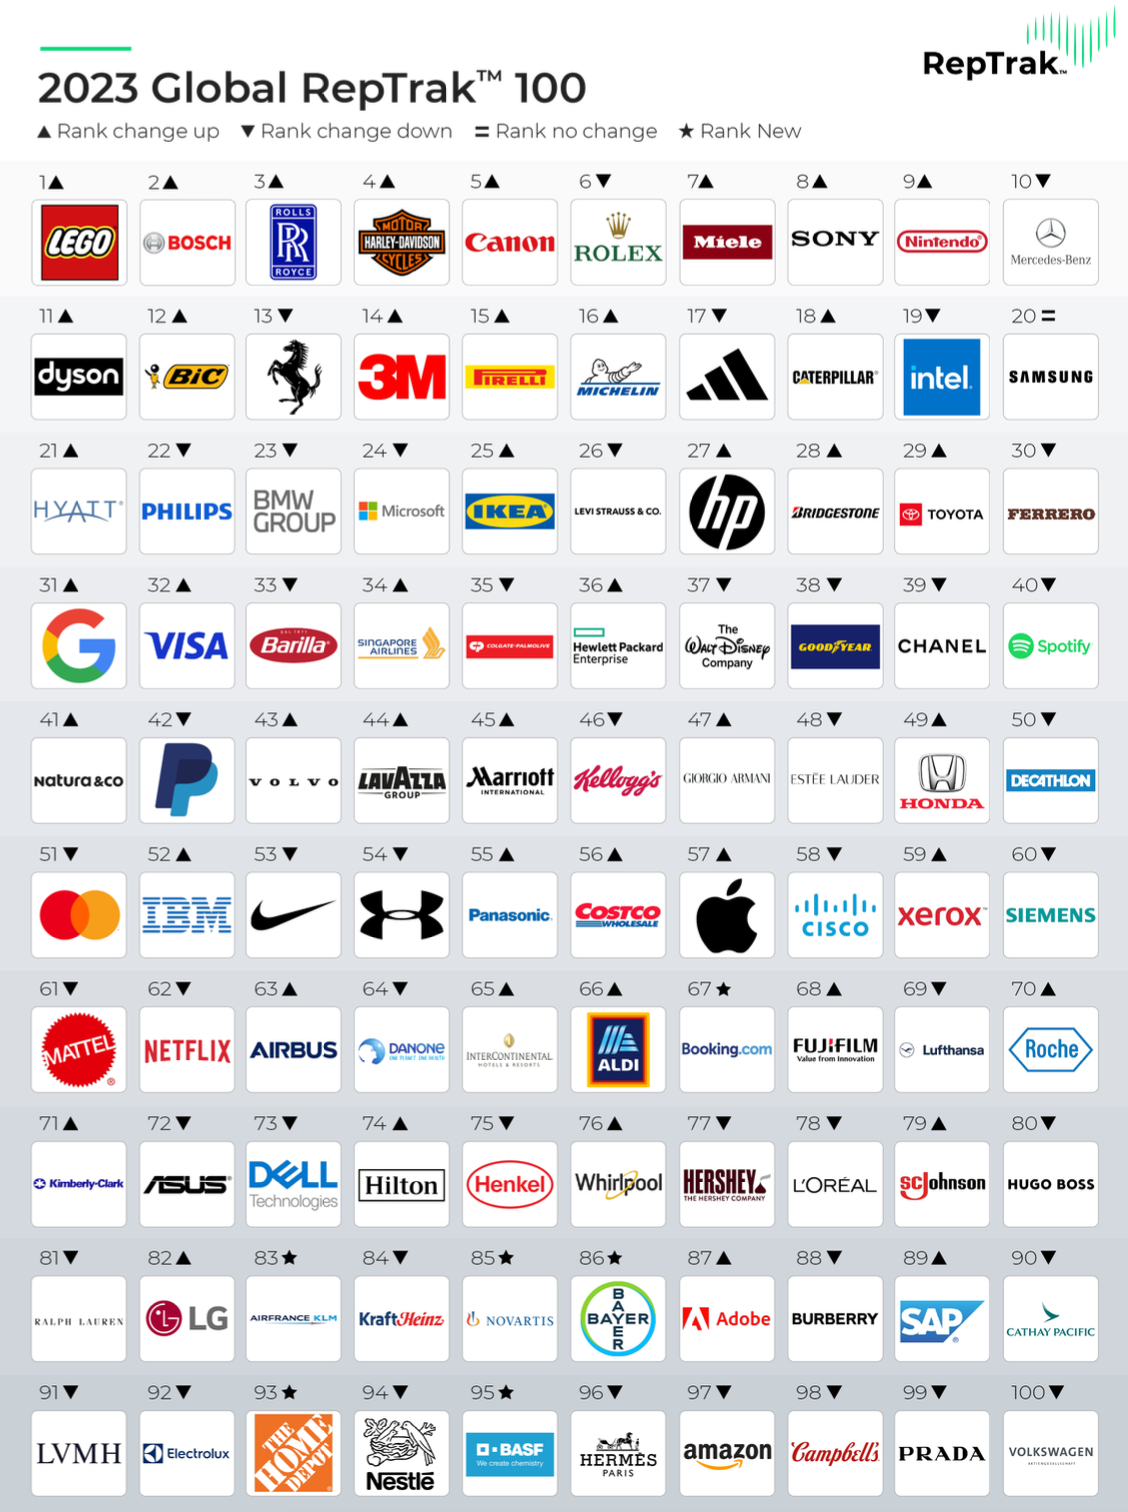
\includegraphics[scale=.85]{assets/images/reptrak-top-100.png}
\end{center}

\section{Les sites les plus consultées}



\chapter{Analyse détaillée}

% L'objectif de cette section est d'analyser en détail les sites web des marques les plus appréciées et les plus consultées pour évaluer leur accessibilité.\\

% \underline{Contenu :} Nous examinerons la conception et les fonctionnalités des sites web des marques les plus appréciées et les plus consultées afin de déterminer si elles sont accessibles à tous. Cela nous permettra de déduire si l'appréciation d'une marque (sa réputation) découle de son accessibilité numérique.\\

% \underline{Conclusions intermédiaires :} À la fin de cette section, nous aurons établi si l'accessibilité numérique contribue à l'appréciation d'une marque, en mettant en évidence des exemples concrets de sites web analysés.\\

\newpage
\chapter{Conclusion}

% L'objectif de cette section est de tirer des conclusions sur la relation entre l'accessibilité numérique et la réputation d'une marque, basées sur les analyses réalisées.\\

% \underline{Contenu :} Nous synthétiserons les résultats obtenus dans les sections précédentes pour répondre à la question centrale. Nous discuterons des implications de notre étude et proposerons des recommandations pour les entreprises afin d'améliorer leur réputation par le biais de l'accessibilité numérique.\\

% \underline{Conclusions finales :} À la fin de ce rapport, nous aurons apporté des éclaircissements sur la relation entre l'accessibilité numérique et la réputation des marques, offrant ainsi des perspectives importantes pour les acteurs du marché.\\

\nocite{*}
\printbibliography[heading=bibintoc,title=Bibliographie]

% L'objectif de cette section est de répertorier les sources utilisées pour étayer notre recherche. À la fin de ce rapport, la bibliographie servira de référence pour les lecteurs intéressés à approfondir le sujet et soulignera la rigueur académique de notre démarche.\\

% \underline{Contenu :} Nous présenterons une liste complète des ouvrages, articles, et ressources en ligne consultés dans le cadre de notre étude. Cela renforcera la crédibilité de nos conclusions en montrant que notre travail s'appuie sur une base solide de connaissances existantes.\\

\makeutbmbackcover{}
\end{document}
